\documentclass{beamer}

\def\Tiny{\fontsize{6pt}{6pt}\selectfont}
\def\supertiny{\fontsize{4pt}{4pt}\selectfont}

\mode<presentation>
{
  \usetheme{Warsaw}
  % \setbeamercovered{transparent}
  \usecolortheme{crane}
}


\usepackage{graphicx, ifthen, listings}

\usepackage[czech]{babel}
% \usefonttheme{professionalfonts}
\usepackage{times}
\usepackage{amsmath}
\usepackage[utf8]{inputenc}
\usepackage{wrapfig}

\usepackage[T1]{fontenc}

\lstset{ basicstyle=\tiny, stringstyle=\ttfamily, showstringspaces=false }

\everymath{\displaystyle}

\setbeamerfont{frametitle}{size=\large}
\setbeamerfont{subsection in toc}{size=\scriptsize}

\makeatletter\newenvironment{blackbox}{%
   \begin{lrbox}{\@tempboxa}\begin{minipage}{0.95\columnwidth}}{\end{minipage}\end{lrbox}%
   \colorbox{black}{\usebox{\@tempboxa}}
}\makeatother

\title[IMF (1)]{Informatika pro moderní fyziky (1)\\základy automatizace; jednoduché zpracování a vizualizace dat}

\author[Franti\v{s}ek HAVL\r{U}J, ORF ÚJV Řež]{Franti\v{s}ek HAVL\r{U}J\\{\scriptsize \emph{e-mail: haf@ujv.cz}}}

\date{zimní semestr 2017/2018\\11. října 2017}

\institute[ORF ÚJV Řež]
{ÚJV Řež\\oddělení Reaktorové fyziky a podpory palivového cyklu}

\AtBeginSection[]
{
\begin{frame}<beamer>
\frametitle{Obsah}
\tableofcontents[currentsection,hideothersubsections]
\end{frame}
}

\begin{document}

\begin{frame}
  \titlepage
\end{frame}

\begin{frame}
  \tableofcontents
\end{frame}

\section{Úvod}

\subsection{Sylabus semináře}

\begin{frame}{Profil absolventa předmětu}
  \begin{itemize}
    \item chápe počítač nikoli jako psací stroj anebo černou skříňku pro specializované aplikace, ale především jako flexibilní a vysoce univerzální nástroj pro každodenní úkoly ve zpracování dat, jejich prezentaci a tvorbě dokumentů
    \item orientuje se v~moderních paradigmatech praktické informatiky, programování na úrovni běžných skriptů je pro něj samozřejmostí a díky solidnímu přehledu je schopen se v~daném problému zorientovat a vybrat si pro jeho řešení vhodný nástroj
    \item není nucen vykonávat mechanickou a nudnou činnost, ale úkoly řeší kreativně - raději si ad hoc vytvoří na míru šitý skript, který jej ochrání před lidskou chybou i frustrací z~monotónnosti
  \end{itemize}
\end{frame}

\begin{frame}{Průběh výuky}
  \begin{itemize}
    \item zadání praktické úlohy, jejíž vyřešení je motivací pro obsah lekce
    \item přednáška na probírané téma, poskytující jak teoretický základ, tak přehled konkrétních nástrojů a postupů
    \item samostatná práce na řešení daného problému
    \item společná diskuse nad jednotlivými řešeními a jejich zhodnocení
  \end{itemize}
\end{frame}

\subsection{K čemu je počítač?}

\begin{frame}{K čemu je počítač?}
  \begin{columns}
    \column{0.6\textwidth}
    \begin{itemize}
      \item počítače udělají cokoliv, pokud na to existuje postup
      \item pokud na něco existuje postup, není na to potřeba člověk
      \item existuje-li postup, existuje také algoritmus
      \item kdo má algoritmus, může napsat program
    \end{itemize}
    \column{0.4\textwidth}
    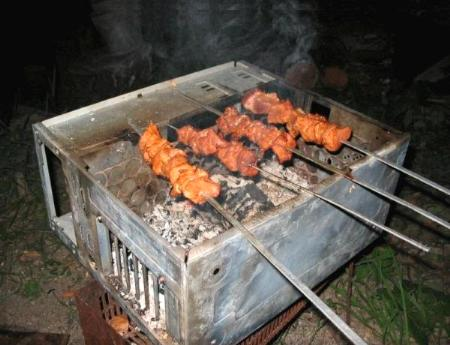
\includegraphics[width=\columnwidth]{computerbarbie}
  \end{columns}
\end{frame}

\begin{frame}{Proč se zabývat automatizací?}
  \begin{columns}
    \column{0.6\textwidth}
    \begin{itemize}
      \item mechanická práce je otravná
      \item program neudělá (náhodnou) chybu
      \item skript trvá stejně dlouho pro libovolný objem dat
      \item pokud je potřeba něco pozměnit nebo jen zpracování zopakovat, je ruční práce vepsí
    \end{itemize}
    \column{0.4\textwidth}
    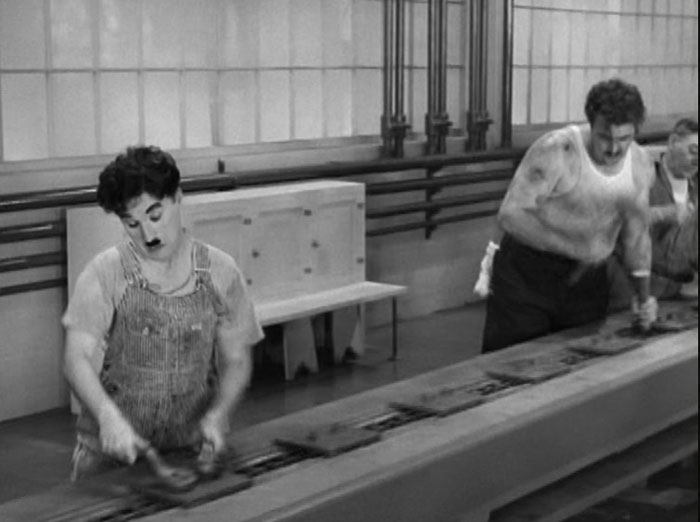
\includegraphics[width=\columnwidth]{chaplin}
  \end{columns}
\end{frame}

\subsection{Problém č. 1: vykreslování dat z~detektoru}

\begin{frame}{Zadání}
  \begin{block}{\# 1}
    Na konci provozní směny je potřeba vyhodnotit signály ze čtyř detektorů a vykreslit je do grafu (signál v~závislosti na čase). Data dostáváte v~jednoduchém textovém souboru (dva sloupce, spousta řádků). Je potřeba vykreslit do jednoho grafu všechny čtyři detektory. Potíž je, že taková data přicházejí každý den - tento úkol je tedy potřeba řešit opakovaně.
  \end{block}
  \begin{block}{S hvězdičkou}
    Počet detektorů je proměnný (1 až 9).
  \end{block}
\end{frame}

\begin{frame}{Příklad}
  \begin{center}
      \includegraphics[width=0.6\columnwidth]{plot4}
      \end{center}

\end{frame}

\subsection{Problém č. 2: jehla v kupce sena}

\begin{frame}{Zadání}
  \begin{block}{\# 2}
    Adresář plný CSV souborů (stovky souborů) obsahuje data, která jsou záznamy signálů s lineární závislostí.

    V pěti z nich jsou ale poruchy - data ležící zcela mimo přímku.

    Kde?
  \end{block}
\end{frame}

\begin{frame}{Příklad - dobrý signál}
  \begin{center}
      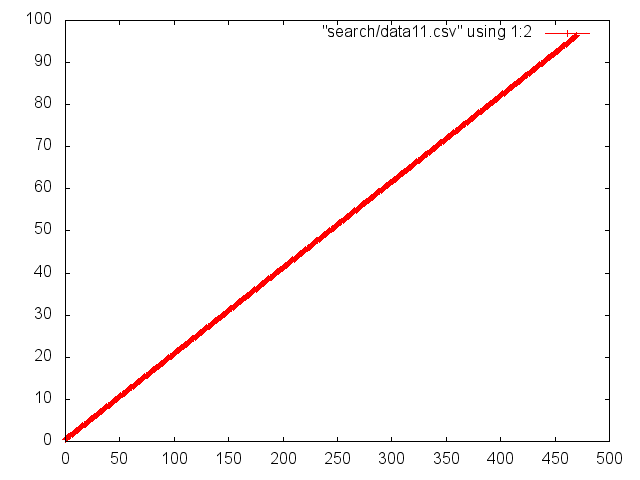
\includegraphics[width=0.6\columnwidth]{search_good}
      \end{center}
\end{frame}
\begin{frame}{Příklad - špatný signál}
  \begin{center}
      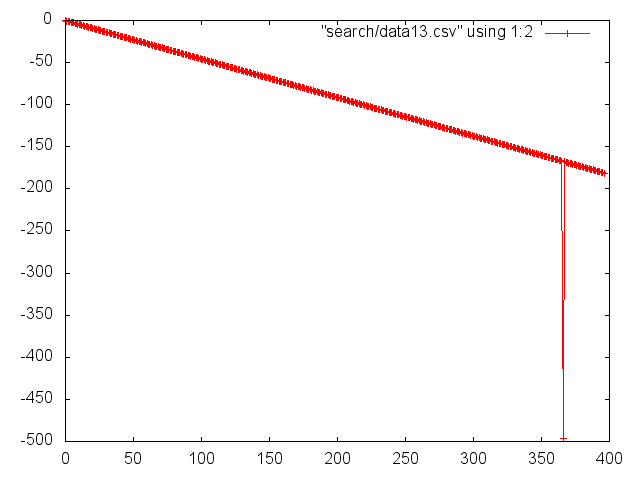
\includegraphics[width=0.6\columnwidth]{search_bad}
      \end{center}
\end{frame}


\subsection{Problém č. 3: zmatek v laborce}

\begin{frame}{Zadání}
  \begin{block}{\# 3}
    V jedné tabulce máme seznam vzorků půdy, jejich datum pořízení a místo odběru, v jiné potom datum měření a naměřené aktivity.

    To všecho musíme dostat dohromady a dopočítat se původní aktivity vzorků v době jejich odběru.

    Do toho je potřeba výsledky nějak dostat do excelu. Navíc bychom se možná rádi trochu předvedli a vzorky zakreslili do mapy.
  \end{block}
\end{frame}

\subsection{Problém č. 4: mnoho výpočtů, inženýrova smrt}

\begin{frame}{Zadání}
  \begin{block}{\# 4}
    Při přípravě základního kritického experimentu je pomocí MCNP potřeba najít kritickou polohu regulační tyče R2.

    Jak se tato poloha změní při změně polohy tyče R1?
  \end{block}
\end{frame}

\section{Ruční a poloautomatická řešení}

\subsection{Problém č. 1: rozbor situace}

\begin{frame}[fragile]{Vstupní data}
  \begin{columns}
    \column{0.7\textwidth}
      {\scriptsize
      \begin{verbatim}
0.00000e+00 0.00000e+00
1.00000e-04 1.01447e-03
2.00000e-04 4.62446e-04
3.00000e-04 6.92465e-04
4.00000e-04 4.48142e-03
5.00000e-04 6.95896e-03
6.00000e-04 5.12501e-03
7.00000e-04 2.62076e-03
...
      \end{verbatim}
      }
    \column{0.29\textwidth}
      \begin{block}{Formát CSV}
        $\bullet$ comma separated values

        $\bullet$ zobecnělo ale jako libovolný formát po sloupcích uložených dat

        $\bullet$ dobře se zpracovává, importuje do Excelu atd.
      \end{block}
  \end{columns}
\end{frame}

\begin{frame}{Klasické řešení (MS Excel)}
  \begin{itemize}
    \item jaké všechny kroky je potřeba udělat?
    \item na který z~provedených kroků byl potřeba člověk -- co z~toho by nemohl stejně dobře udělat počítač sám?
    \item jaké jsou výhody a nevýhody ručního řešení?
    \item jak by mělo takové automatické řešení fungovat?
  \end{itemize}
\end{frame}

\begin{frame}{Co by takové automatické řešení mohlo umět?}
  \begin{itemize}
    \item načte z daného adresáře soubory se záznamy
    \item vykreslí graf a uloží ho do souboru
    \item soubor jednoznačně pojmenuje a zkopíruje na vhodné místo
    \item uživatel by neměl v ideálním případě dělat vůbec nic
  \end{itemize}
\end{frame}

\begin{frame}{Komponenty pro automatizaci}
  \begin{block}{Funkční části}
    výkonné programy (např. kreslení grafů, generování tabulek/reportů, spouštění výpočtů) -- předpokladem je možnost spouštět program v~neinteraktivním (dávkovém) režimu
  \end{block}
  \pause
  \begin{block}{Jak to slepit dohromady}
    dávkový soubor (BAT) nebo skript -- je nutno vždy vhodně volit použité prostředky ve vztahu k~jednoduchosti, požadavkům na funkce, přenositelnosti
  \end{block}
\end{frame}

\begin{frame}{Jak postupovat s~automatickým řešením?}
  \begin{enumerate}
    \item vykreslit graf s~jedním detektorem
    \pause
    \item se všemi detektory
    \pause
    \item z~příkazové řádky
    \pause
    \item z~batch souboru
    \pause
    \item se jménem adresáře jako parametrem
  \end{enumerate}
\end{frame}

\begin{frame}{Gnuplot}
  \begin{columns}
    \column{0.7\textwidth}
      \begin{itemize}
        \item interaktivní i dávkový režim -- ideální pro automatizaci
        \item slušně konfigurovatelné 2D i 3D grafy
        \item i bez nastavení funguje velmi přijatelně
        \item široká paleta výstupních formátů
      \end{itemize}
    \column{0.29\textwidth}
      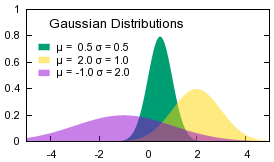
\includegraphics[width=\columnwidth]{gnuplot1}

      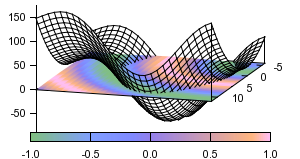
\includegraphics[width=\columnwidth]{gnuplot2}
  \end{columns}
\end{frame}

\subsection{Řešení}

\begin{frame}[fragile]{Vykreslení jednoho grafu v~gnuplotu}
  \begin{verbatim}
    gnuplot> plot "data1.csv"
  \end{verbatim}
  \pause
  \begin{center}
    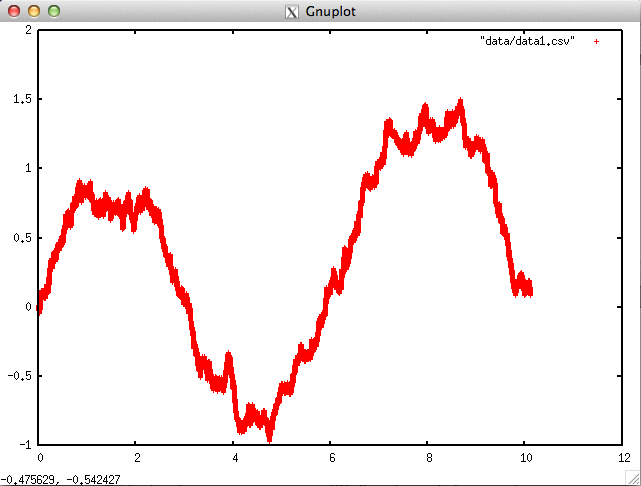
\includegraphics[width=0.6\textwidth]{gnuplot_interactive}
  \end{center}
\end{frame}

\begin{frame}[fragile]{Vykreslení všech grafů v~gnuplotu}
  \begin{verbatim}
    gnuplot> plot "data1.csv", "data2.csv",
                  "data3.csv", "data4.csv"
  \end{verbatim}
  \pause
  \begin{center}
    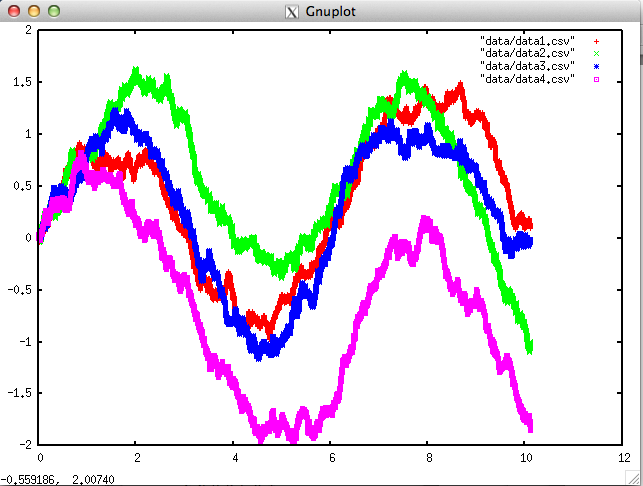
\includegraphics[width=0.6\textwidth]{gnuplot_interactive_all}
  \end{center}
\end{frame}

\begin{frame}[fragile]{Dávkové použití}
  \scriptsize
  \begin{verbatim}
    set terminal png
    set output "plot4.png"
    plot "data/data1.csv", "data/data2.csv", \
         "data/data3.csv", "data/data4.csv"
  \end{verbatim}
  \pause
  \begin{center}
    \includegraphics[width=0.6\textwidth]{../gnuplot/plot4}
  \end{center}
\end{frame}

\begin{frame}[fragile]{BAT soubor}
  Je pracné pokaždé vypisovat parametry na příkazovou řádku. .BAT soubory ve Windows fungují jednoduše, prostě se do nich dá psát jako do terminálu a připravit si tak jednodušší skript.
  \begin{verbatim}
    gnuplot plot.gp
  \end{verbatim}
\end{frame}

\begin{frame}[fragile]{BAT soubor s~parametrem}
  Co takhle adresář pro každý den? Nemá smysl pokaždé ručně kopírovat vstup pro gnuplot a tak dále...

  Stačí vědět, že BAT soubor může mít na příkazové řádce parametry. První parametr je uložen do proměnné \texttt{\%1} a to se nám bude hodit.

  \begin{verbatim}
    cd %1
    gnuplot ../plot.gp
    cd ..
  \end{verbatim}
\end{frame}

\begin{frame}[fragile]{BAT soubor s~parametrem - vylepšení}
  Pokud si budeme chtít prohlédnout grafy, bude nutné vždy vlézt do adresáře a otevřít \texttt{plot.png}. Jde to ovšem vylepšit pomocí jednoduchého triku:

  \begin{verbatim}
    cd %1
    gnuplot ../plot.gp
    copy plot.png ../%1.png
    cd ..
  \end{verbatim}
\end{frame}

\subsection{Zhodnocení}

\begin{frame}{Jak moc jsme si pomohli?}
  \begin{itemize}
    \item jeden skript místo excelovské anabáze
    \item máme znovupoužitelný nástroj -- můžeme proces kdykoliv zopakovat
    \item nelze udělat žádnou ``ruční chybu''
    \item skript můžeme dát kolegovi a ten má práci hotovou úplně zadarmo
    \item skript lze periodicky spouštět bez účasti uživatele, možnost např. zobrazovat na intranetu aktuální grafy atd.
  \end{itemize}
\end{frame}

\subsection{Problém č. 2, 3, 4: jak na to?}

\begin{frame}{Stačí nám to na řešení problému č. 2, 3, 4?}
  Zatím nevíme, jak:
  \begin{itemize}
    \item prohledat adresář a vygenerovat spoustu grafů
  \end{itemize}
  \begin{itemize}
    \item pospojovat data ze dvou souborů a navrch něco vypočítat, co teprv zakreslit to do mapy
  \end{itemize}
  \begin{itemize}
    \item vygenerovat vstupní soubory pro MCNP
    \item spustit hromadu MCNP výpočtů
    \item vytahat výsledky z~MCNP výstupního souboru
  \end{itemize}
  Budeme potřebovat nějaký těžší kalibr.
\end{frame}

\section{Skriptovací jazyky}

\subsection{Úvod do skriptování}

\begin{frame}{``klasické'' programování -- Pascal, C++}
  \begin{itemize}
    \item napsat zdroják, zkompilovat, slinkovat ...
    \item ... muset řešit binárku, která někde funguje a někde ne ...
    \item ... moc práce!
    \item (i když výhody jsou zřejmé -- rychlost, distribuce binárek místo zdrojáků, ``uzavřené'' prostředí)
    \item bylo by lepší mít někdy místo motorové pily sekeru
  \end{itemize}
\end{frame}

\begin{frame}{Interpretované jazyky / skripty}
  \begin{itemize}
    \item textový vstupní soubor (zdrojový kód) + interpret
    \item vhodné pro aplikace bez vysokých nároků na systém
    \item nebo tam, kde je zásadní snížit nároky na vývoj
    \item tj. ideální pro jednoúčelové a krátkodobě žijící programy
    \item většinou ``volnější'' pojetí programování, z~čehož plyne například řádově elegantnější práce s~textem
  \end{itemize}
\end{frame}

\begin{frame}{Vlastnosti skriptovacích jazyků}
  \begin{block}{Výhody}
    \begin{itemize}
      \item dokonalá přenositelnost (textové vstupní soubory)
      \item nic se nekompiluje
      \item většinou syntakticky úsporné
    \end{itemize}
  \end{block}
  \pause
  \begin{block}{Nevýhody}
    \begin{itemize}
      \item zdrojový kód je otevřený (ne vždy se to hodí)
      \item pomalé a paměťově náročné
      \item bez kontroly správnosti při kompilaci
    \end{itemize}
  \end{block}
\end{frame}

\begin{frame}{Přehled hlavních jazyků}
  \begin{description}
    \item[BAT] -- vhodné pouze pro to nejjednodušší použití; i když jsou k~mání některé trochu složitější funkce, jejich použití je hodně neobratné a neefektivní
    \item[BASH] -- podstatně mocnější alternativa BAT souborů v~prostředí Unixu; nepříliš intuitivní syntaxe a absence náročnějších operací
    \item[Perl] -- kompaktní a efektní jazyk, který je všude nainstalovaný, ale nedá se (vůbec) číst a už i pole apod. jsou nekřesťansky obskurní
    \item[Python] -- velmi slušný jazyk, který snese i ``vážnější'' využití, ale za cenu trochu vyšší obtížnosti
    \item[Ruby] -- elixír síly a zázračná pilulka: intuitivní, snadný, všemocný, rozšířený a k~tomu ryze objektový
  \end{description}
\end{frame}

\subsection{Úvod do jazyka Ruby}

\begin{frame}{Jazyk Ruby}
  \begin{itemize}
    \item čistě objektový interpretovaný jazyk
    \item interprety existují pro širokou škálu platforem
    \item velmi elegantní syntaxe
    \item nevýhodou je stále ještě relativní pomalost
    \item aktuální verze 2.2 (rozumné minimum je 1.9.3, míň nebrat)
  \end{itemize}
\end{frame}

\begin{frame}[fragile]{Ukázka Ruby (1)}
  Každý programátor tím začíná ...
  \begin{block}{}
    \smallskip \footnotesize
    {\scriptsize \begin{verbatim}
      puts "Hello world!"
    \end{verbatim}}
  \end{block}
  \pause
  \begin{block}{}
    \smallskip \footnotesize
    {\scriptsize \begin{verbatim}
      Hello world!
    \end{verbatim}}
  \end{block}
\end{frame}

\begin{frame}[fragile]{Ukázka Ruby (2)}
  Proměnné, \texttt{print} vs. \texttt{puts}, aritmetika
  \begin{block}{}
    \smallskip \footnotesize
    {\scriptsize \begin{verbatim}
      a = 4
      b = 5
      print "4 + 5 = "
      puts a + b
    \end{verbatim}}
  \end{block}
  \pause
  \begin{block}{}
    \smallskip \footnotesize
    {\scriptsize \begin{verbatim}
      4 + 5 = 9
    \end{verbatim}}
  \end{block}
\end{frame}

\begin{frame}[fragile]{Ukázka Ruby (3)}
  In-line výrazy v~řetězcích
  \begin{block}{}
    \smallskip \footnotesize
    {\scriptsize \begin{verbatim}
      a = 4
      b = 5
      puts "#{a} + #{b} = #{a+b}"
    \end{verbatim}}
  \end{block}
  \pause
  \begin{block}{}
    \smallskip \footnotesize
    {\scriptsize \begin{verbatim}
      4 + 5 = 9
    \end{verbatim}}
  \end{block}
\end{frame}

\begin{frame}[fragile]{Důležitá vsuvka}
  Řetězec
  \begin{block}{}
    \smallskip \footnotesize
    {\scriptsize \begin{verbatim}
      "a"
    \end{verbatim}}
  \end{block}
  \pause
  Proměnná
  \begin{block}{}
    \smallskip \footnotesize
    {\scriptsize \begin{verbatim}
      a
    \end{verbatim}}
  \end{block}
  \pause
  Řetězec s proměnnou uvnitř
  \begin{block}{}
    \smallskip \footnotesize
    {\scriptsize \begin{verbatim}
      "#{a}"
    \end{verbatim}}
  \end{block}
\end{frame}

\begin{frame}[fragile]{Ukázka Ruby (4)}
  Rozsahy a cykly
  \begin{block}{}
    \smallskip \footnotesize
    {\scriptsize \begin{verbatim}
      (1..5).each do |i|
        puts "#{i} * #{i} = #{i * i}"
      end
    \end{verbatim}}
  \end{block}
  \pause
  \begin{block}{}
    \smallskip \footnotesize
    {\scriptsize \begin{verbatim}
      1 * 1 = 1
      2 * 2 = 4
      3 * 3 = 9
      4 * 4 = 16
      5 * 5 = 25
    \end{verbatim}}
  \end{block}
\end{frame}


\begin{frame}[fragile]{Ukázka Ruby (4)}
  Pětkrát nic umořilo osla (opakování, ne cyklus)
  \begin{block}{}
    \smallskip \footnotesize
    {\scriptsize \begin{verbatim}
      5.times do
        puts "nic"
      end
    \end{verbatim}}
  \end{block}
  \pause
  \begin{block}{}
    \smallskip \footnotesize
    {\scriptsize \begin{verbatim}
      nic
      nic
      nic
      nic
      nic
    \end{verbatim}}
  \end{block}
\end{frame}

\subsection{První kroky s~Ruby}

\begin{frame}[fragile]{IRb}
  Pro první ozkoušení (a i pro některé úkoly v~praktickém životě) se hodí ``příkazová řádka'' Ruby, tzv. \textbf{Interactive Ruby} (\texttt{IRb}):
  \pause
  \begin{block}{}
    {\scriptsize \begin{verbatim}
      1.9.2-p290 :001 > 2+2
       => 4
      1.9.2-p290 :002 > a = 5
       => 5
      1.9.2-p290 :003 > b = 6
       => 6
      1.9.2-p290 :004 > a * b
       => 30
    \end{verbatim}}
  \end{block}

\end{frame}

\begin{frame}[fragile]{Proměnné, výpis na terminál}
  V Ruby (jak je u skriptů zvykem) se proměnné nedeklarují:
  \begin{block}{}
    {\scriptsize \begin{verbatim}
      a = 5
      a = a * a
      long_string = "looooong string"
    \end{verbatim}}
  \end{block}
  \pause
  Výpis se děje pomocí print, resp. puts (bez/s~koncem řádku); \texttt{\#\{...\}} vkládá do řetězce libovolný výraz:
  \begin{block}{}
    {\scriptsize \begin{verbatim}
      print a
      puts "a = #{a}"
    \end{verbatim}}
  \end{block}
\end{frame}

\begin{frame}[fragile]{Pole a hashe}
  Pole je seznam:
  \begin{block}{}
    {\scriptsize \begin{verbatim}
      a = []
      a << 5
      a += [6]
      puts a.size
    \end{verbatim}}
  \end{block}
  \pause
  Hash, neboli slovník či asociativní pole:
  \begin{block}{}
    {\scriptsize \begin{verbatim}
      b = {}
      b[3] = 7
      b["foo"] = "bar"
    \end{verbatim}}
  \end{block}
\end{frame}

\begin{frame}[fragile]{Rozsahy a cykly}
  Rozsahy (ranges) - se dvěma tečkami včetně posledního elementu, se třemi bez něj
  \begin{block}{}
    {\scriptsize \begin{verbatim}
      a = (1..5)
      b = (1...5)
      puts "yay!" if a.size == b.size + 1
    \end{verbatim}}
  \end{block}
  \pause
  Ruby nepoužívá klasický cyklus, ale iterátor (přes téměř cokoliv):
  \begin{block}{}
    {\scriptsize \begin{verbatim}
      (1..5).each do |i|
        puts i * i
      end
      b = {}; b["key1"] = 6; b["key2"] = 8
      b.each do |key, value|
        puts "#{key} => #{value}"
      end
    \end{verbatim}}
  \end{block}
\end{frame}

\begin{frame}[fragile]{Práce s~řetězci, include, split, sub}
  Řetězce v~Ruby jsou neomezené délky (pár mega se tam určitě vejde) a dá se s~nimi provádět ledacos.
  \begin{block}{}
    {\scriptsize \begin{verbatim}
      s = "lazy dog"
      if s.include?("lazy")
        puts "lazy!!!"
      end
    \end{verbatim}}
  \end{block}
  \pause
  Rozdělit? Nahradit?
  \begin{block}{}
    {\scriptsize \begin{verbatim}
      puts s.sub("lazy", "crazy")
      a = s.split
      puts "#{a[1]} #{a[0]}"
    \end{verbatim}}
  \end{block}
\end{frame}

\begin{frame}[fragile]{Načítání a zápis do souboru}
  Soubor a terminál, to je vlastně jedno:
  \begin{block}{}
    {\scriptsize \begin{verbatim}
      File.open("animals.txt", "w") do |f|
        f.puts "quick brown fox"
      end
    \end{verbatim}}
  \end{block}
  \pause
  Nejjednodušší čtení je po řádcích:
  \begin{block}{}
    {\scriptsize \begin{verbatim}
      IO.foreach("data.csv") do |line|
        ...
      end
    \end{verbatim}}
  \end{block}
\end{frame}

\begin{frame}[fragile]{Práce s~adresářem}
  Jak projít všechny soubory v~adresáři? V Pascalu utrpení, v~Ruby iterátor:
  \begin{block}{}
    {\scriptsize \begin{verbatim}
      Dir["*"].each do |filename|
        puts filename
      end
    \end{verbatim}}
  \end{block}
  \pause
  Lze použít podle očekávání libovolnou masku nebo cestu:
  \begin{block}{}
    {\scriptsize \begin{verbatim}
      Dir["data/*.csv"].each do |filename|
        IO.foreach(filename) do |line|
          puts line
        end
      end
    \end{verbatim}}
  \end{block}
\end{frame}

\begin{frame}{A to je vše, přátelé!}
  \begin{center}
    
\includegraphics[width=0.7\textwidth]{looney_tunes}
  \end{center}
\end{frame}

\begin{frame}{Příště}
  \begin{block}{Ruby}
    \begin{itemize}
      \item opakování a drobná cvičení
      \item více o čtení souborů a výstupu na terminál
    \end{itemize}
  \end{block}
  \begin{block}{Problém č. 2}
    \begin{itemize}
      \item první skripty
    \end{itemize}
  \end{block}
  \begin{block}{Problém č. 3}
    \begin{itemize}
      \item ukládání dat do vhodných struktur
      \item generování vhodných pohledů a reportů
    \end{itemize}
  \end{block}
\end{frame}

\end{document}
